\section{Results}
The spectra were obtained

[Calibration] was then necessary,
in order [to derive the linear relationship] between [the channels] of the Multi Channel Analyser (MCA) thingy in which signal is detected 
and the corresponding energy values

This was accomplished using the known decay schems of the four sources.

\paragraph{Attenuation [in matter?]}
[We chose Cesium because of its high count rate]

\begin{figure}[htbp]
    \centering
    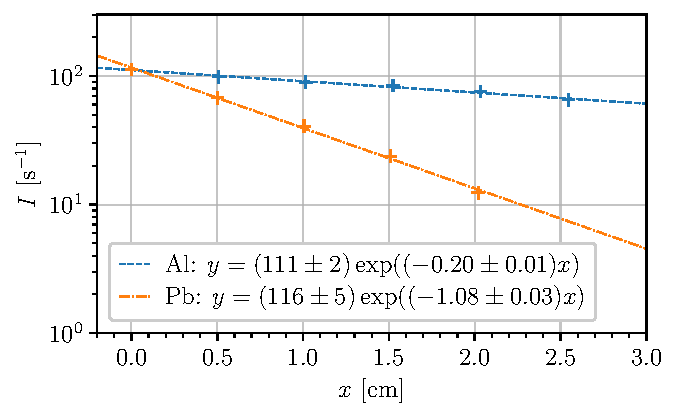
\includegraphics[scale=1]{figures/attenuation_coefficient.pdf}
    \caption{Radiation attenuation through Aluminum (Al) and Lead (Pb). 
             The error bars were omitted in reason of their small relative size 
             (1\% on the intensity and $1$ $\mu$m on the thickness of the material).}
    \label{fig:attenuation_coefficient}
\end{figure}

After obtaining the linear attenuation coefficient it was possible to [get] the energies of the $\gamma$ rays emitted from the source by checking the tables in Annex blabla in \cite{notice_generale}.
The Results are compatible with the previously obtained [or known??] spectrum for the $^{137}$Cs